
%\addcontentsline{toc}{chapter}{\hspace{-0.3in}\protect\numberline{}Appendices}
\appendix
\normalsize
\chapter{Elemental Solution Superposition}

The method of elemental solution superposition can be used to construct the solution of pressure Poisson equation arising from the primitive variables formulation for incompressible flows. However, the complexity for constructing the whole domain solution is $O(N^2)$, which is more expensive compared with $O(N)$ for the multigrid method and $O(N\ log \ N)$ for the fast fourier transform. To reduce the complexity of the superposition method, the whole domain is decomposed into subdomains and the solution is constructed only on the interfaces shared by neighboring subdomains. To further reduce the complexity, the solution is approximated locally, i.e., only the source terms from neighboring nodes contribute to the solution on the interface. After the pressure Poisson solution is constructed on the interface, each subdomain can be solved independently with the newly constructed boundary values. The flow model with this proposed elemental solution superposition method is still under development.



\section{Elemental Solutions and Elemental Boundary Conditions} \label{section-ESS}
The concept of the elemental solution can be traced back to the Green's function \cite{Green1828,Cheng05}, which is the solution to the governing equation with Dirac delta source.

Consider a linear differential equation with Dirichlet, Neumann, and Robin boundary conditions, where $\mathcal{L}$ is the differential operator:
\ba
\mathcal{L} \Phi(r)= S(r) \hst \te{in} \hst \Omega \hst \te{and} \\
\Phi(r)= D(r) \hs{0.2in} \te{on} \hs{0.2in} (\p\Omega)_1 \\
\f{\p\Phi(r)}{\p n} = Q(r) \hs{0.2in} \te{on} \hs{0.2in} (\p\Omega)_2 \\
\alpha \f{\p\Phi(r)}{\p n} + \beta \Phi(r)= R(r) \hs{0.2in} \te{on} \hs{0.2in} (\p\Omega)_3
\ea
The inverse $L$ operator can be defined as an integral operator:
\ba
\mathcal{L}^{-1}S= \int_\Omega E_S(r,r')S(r')dr' + \int_{(\p \Omega)_1} E_D(r,r')D(r')da' \nn\\
+ \int_{(\p \Omega)_2} E_Q(r,r')Q(r')da'
+ \int_{(\p \Omega)_3} E_R(r,r')R(r')da'
\ea
where the elemental solution $E_S$ is defined as the solution to the governing equation with finite volume averaged Dirac delta function; $E_D$, $E_Q$, $E_R$ are the elemental solutions with corresponding elemental boundary conditions on the boundaries. The boundaries of elemental solutions coincide the boundary specified for the governing equation, but the imposed boundary conditions are different from the assigned boundary conditions. Rather, the boundary conditions of elemental solutions are decomposed from the specified boundary conditions and are called "elemental boundary conditions". The decomposition of the boundary condition is based on the boundary discretization or surface meshing as shown in the following examples.

\subsection{Laplace Equation with Dirichlet Boundary Condition}%\label{subsection:Laplace-Dirichlet}

\begin{figure}[htbp]
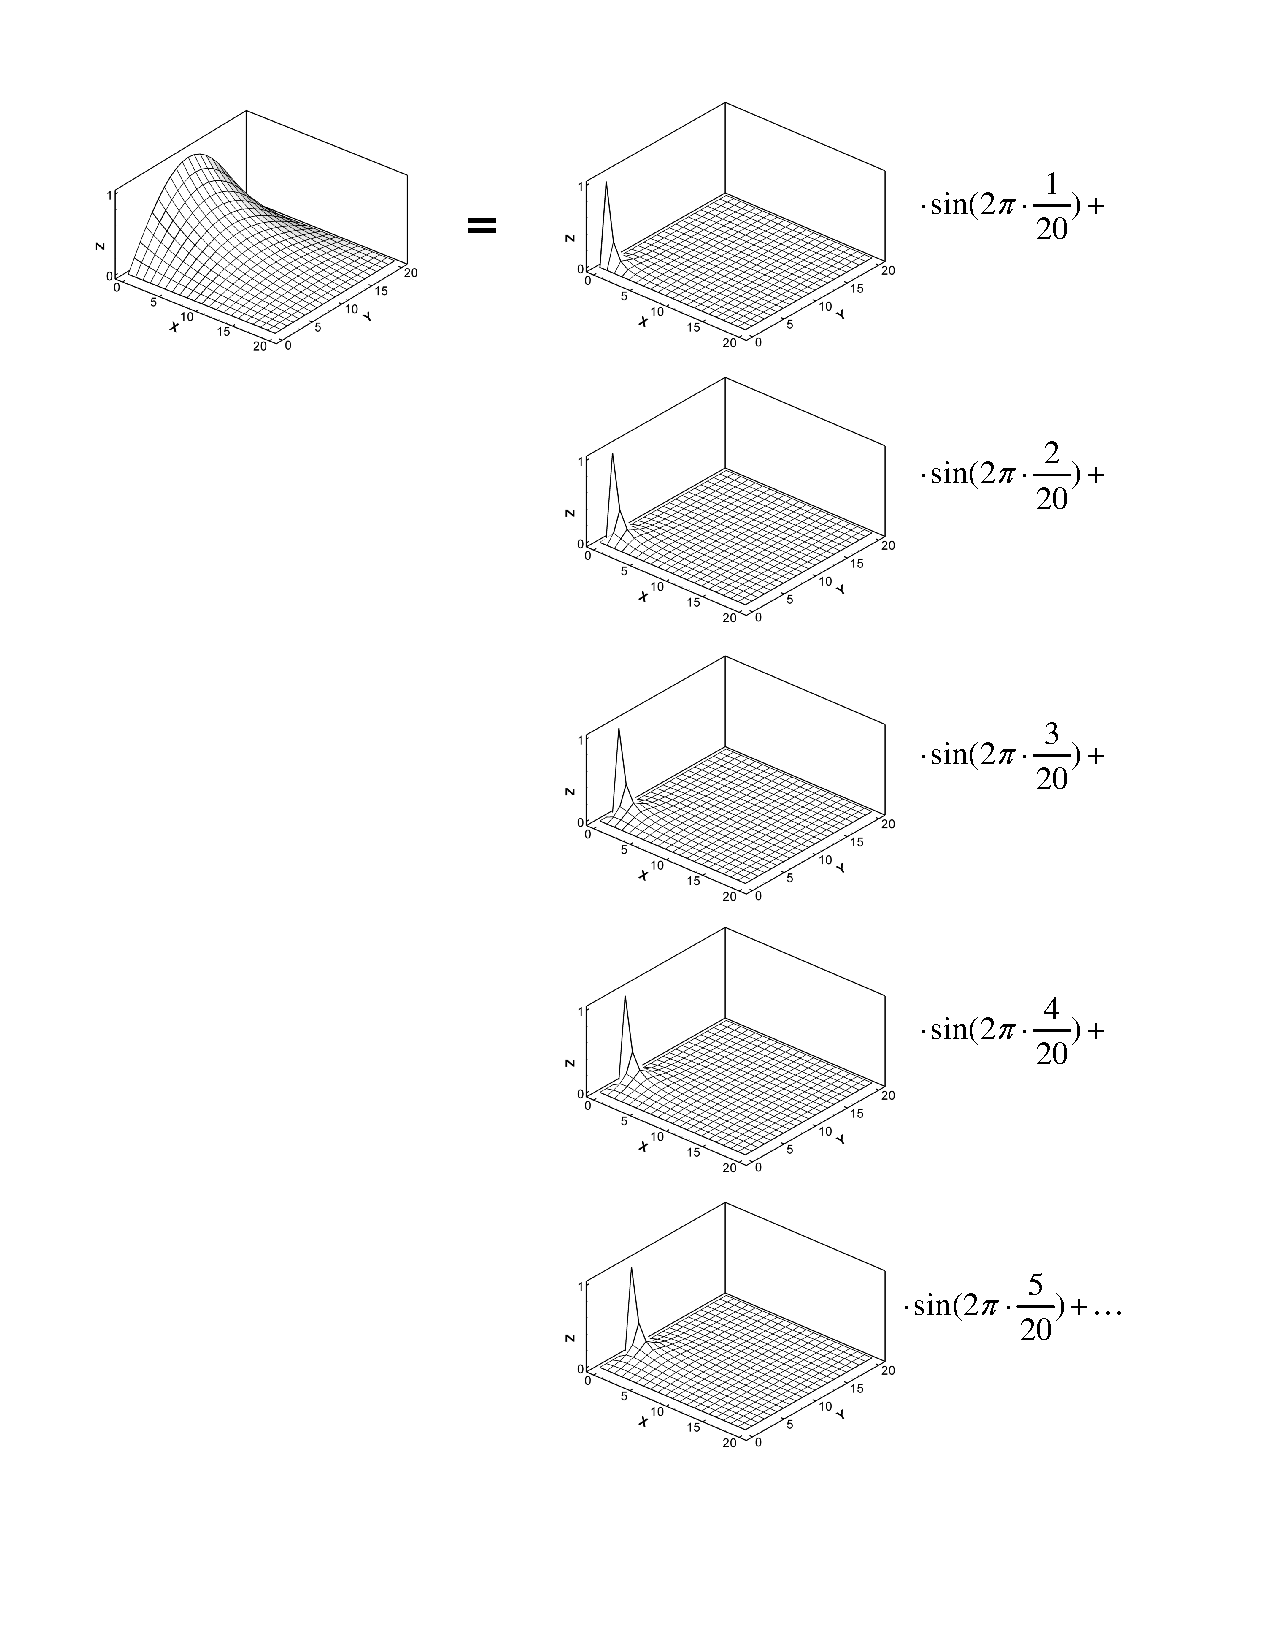
\includegraphics[width=6in]{../figures/SES/example_Laplace.pdf}
\caption{Laplace equation with Dirichlet Boundary Condition}
\label{fig:example-Laplace-Dirichlet}
\end{figure}


Let's consider the superposition technique for the Laplace equation with Dirichlet boundary condition, this is the case that the source term $S$ is zero in the domain $\Omega$ and the value of $\Phi$ is specified on the boundary $\p \Omega$:
\be
\n^2 \Phi(r)= 0 \hst \te{in} \hst \Omega
\hst \te{and} \hst
\Phi(r)= D(r) \hs{0.2in} \te{on} \hs{0.2in} \p\Omega \hs{0.3in}
\label{eqn:Laplace-Dirichlet}
\ee
The finite difference method is used to discretize the above equation such that there are $N$ discrete points inside the domain $\Omega$, and $W$ discrete points on the domain boundary $\p \Omega$. The system of equations resulted from the finite difference method can be written as:
\be
\left[
\baa{cccc}
a_{11} & a_{12} & \ldots & a_{1N} \\
a_{21} & a_{22} & \ldots & a_{2N} \\
\vdots & \vdots & \ddots & \vdots \\
a_{N1} & a_{N2} & \ldots & a_{NN}
\eaa
\right]\left[
\baa{c}
\phi_{1} \\ \phi_{2} \\ \vdots \\
\phi_{N}
\eaa
\right]=
\left[
\baa{c}
b_{1} \\ b_{2} \\ \vdots \\
b_{N}
\eaa
\right]
\ee
or
\be
A  \Phi = B
\ee
The boundary value is discretized into $W$ points as:
\be
D = (d_1, d_2, ....., d_W)^T
\ee
We can choose $W$ sets of fundamental Dirichlet boundaries $D^o_i$, which are zero everywhere except at the $i-th$ point the boundary value equals unity:
\be
D^o_i=( d^o_{i1}, \ d^o_{i2}, \ \cdots, \ d^o_{iW}  ) \hst
d^o_{ij} = \left\{
\baa{ccc}
0 \hst & if & j\neq i \\
1 \hst & if & j= i
\eaa
\right.
\ee
The corresponding numerical fundamental solutions that satisfy the above fundamental boundary conditions can be computed as:
\be
\Phi^o_i = (\phi^o_{i1}, \ \phi^o_{i2}, \ \cdots, \ \phi^o_{iN})^T \\
\ee
According the superposition principle, the general solution for Equation \ref{eqn:Laplace-Dirichlet} can be constructed as:
\be
\left[
\baa{c}
\phi_{1} \\ \phi_{2} \\ \vdots \\
\phi_{N}
\eaa
\right]=\sum_{i=1}^W
d_{i}
\left[
\baa{c}
\phi^o_{i1} \\ \phi^o_{i2} \\ \vdots \\
\phi^o_{iN}
\eaa
\right]
\ee
or
\be
\Phi = \sum_{i=1}^W d_i \Phi^o_i
\ee
Laplace equation in a square domain with a sinusoidal Dirichlet boundary on one side and boundary value equals zero on the others:
\ben
\n^2 \Phi(x,y)=0, \hst 0< x, y <20;
\een
\be
\Phi(0,y)= sin(2 \pi \f{y}{20}),\hst \Phi(20,y)=\Phi(x,0)=\Phi(x,20)=0
\ee
Let $\Delta x=\Delta y=h=1$,
the two-dimensional 5-point central difference approximation of the Poisson equation is
\be
\f{\Phi_{i+1,j}+\Phi_{i-1,j}+\Phi_{i,j+1}+\Phi_{i,j-1}-4\Phi_{i,j}}{ h^2}=0
\ee
where $i$ denotes the grid point index in the $x$ direction and $j$ in the $y$ direction.

The fundamental solution $\Phi^o_j$ is computed by setting the boundary value equals unity at $(x,y)=(0,j\Delta y)$ and equals zero otherwise:
\ben
\n^2 \Phi^o_j(x,y)=0, \hst 0< x, y <20 ; \hst \Phi(20,y)=\Phi(x,0)=\Phi(x,20)=0, \nonumber
\een
\be
\Phi(0,y) = \left\{
\baa{ccc}
0 \hst & if & y\neq j\Delta y \\
1 \hst & if & y = j\Delta y
\eaa
\right.
\ee
The solution $\Phi$ can be constructed by superposing all the fundamental solutions multiplied by the boundary values as shown in Figure \ref{fig:example-Laplace-Dirichlet}

\subsection{Laplace Equation with Neumann Boundary Condition}%\label{subsection:Laplace-Neumann}

\begin{figure}[htbp]
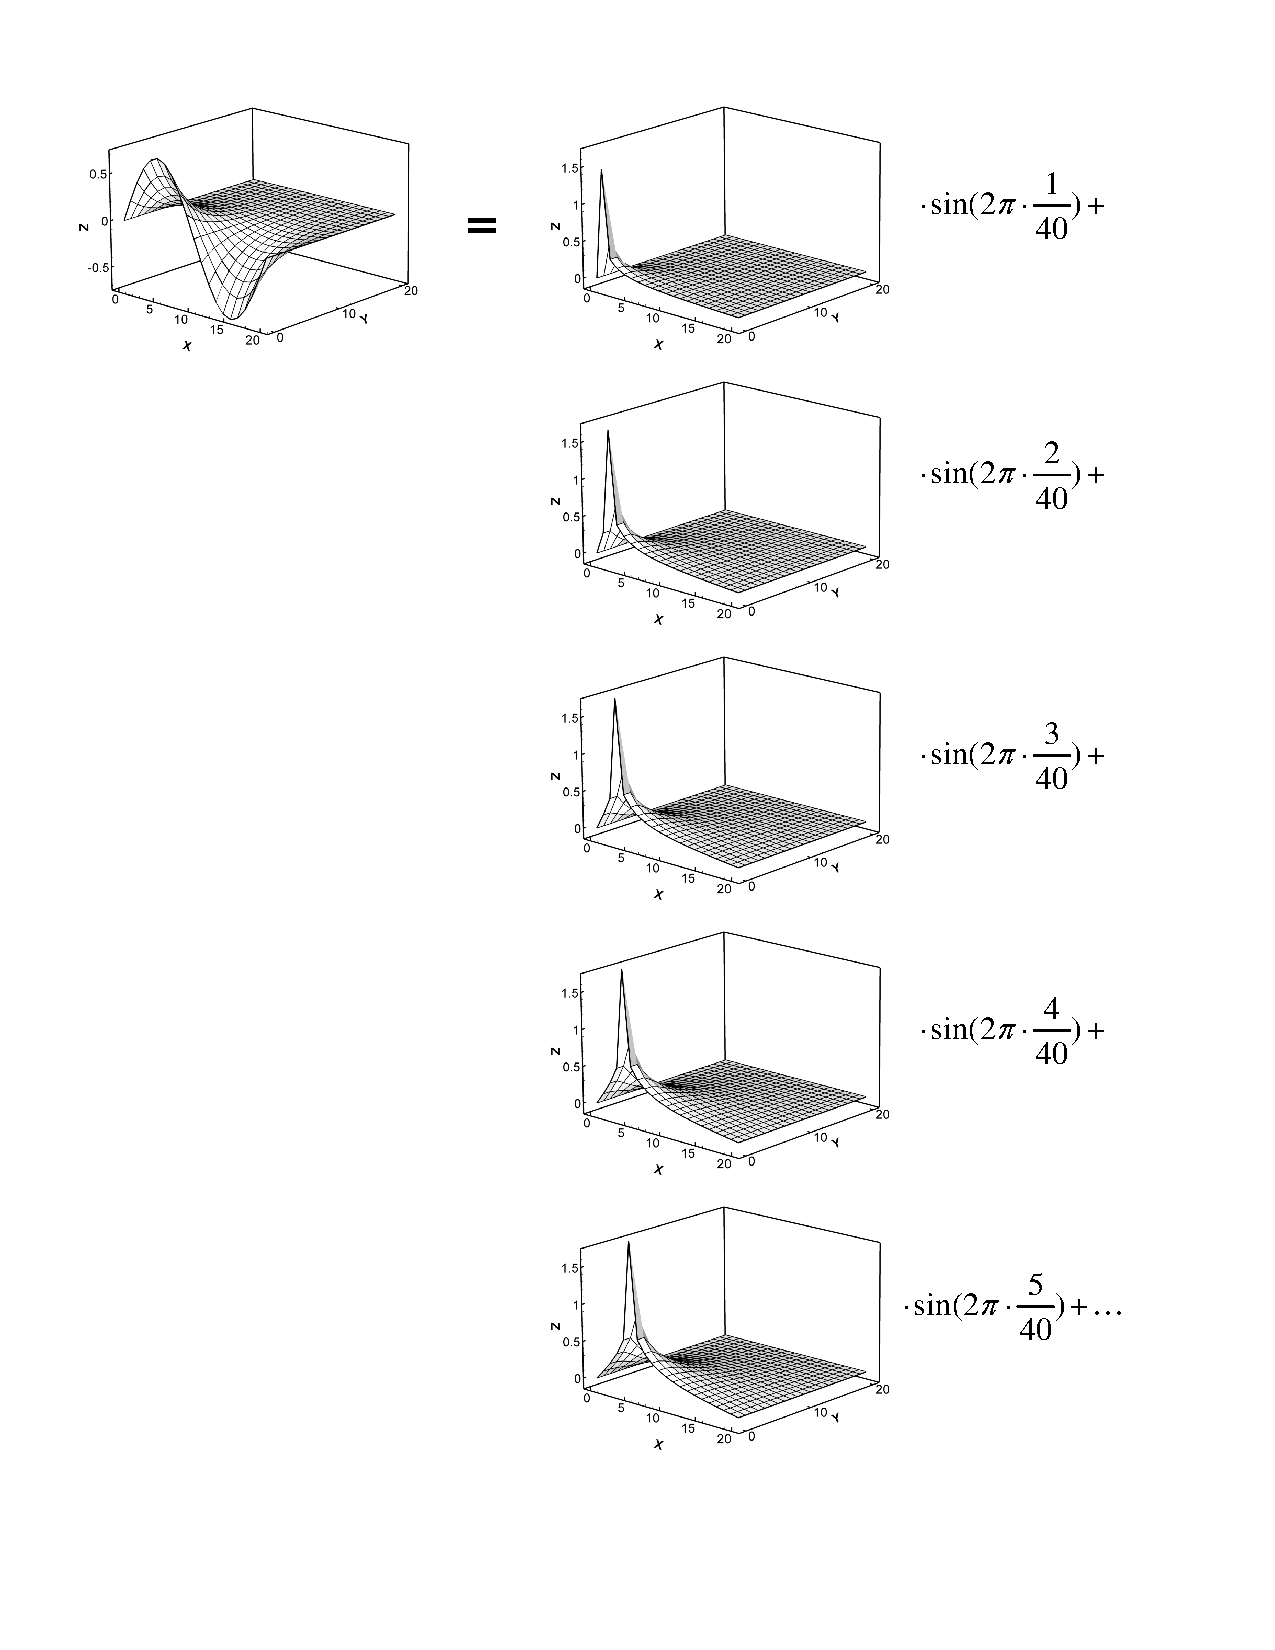
\includegraphics[width=6in]{../figures/SES/example_Neumann.pdf}
\caption{Laplace equation with Newmann boundary condition}
\label{fig:example-Laplace-Neumann}
\end{figure}


After deriving the superposed solution for Laplace equation with Dirichlet Boundary condition, we will next discuss the Neumann boundary condition, where the gradient of the boundary value is specified:
\be
\n^2 \Phi(r)= 0 \hst \te{in} \hst \Omega
\hst \te{and} \hst
\f{\p\Phi(r)}{\p n}= Q(r) \hs{0.2in} \te{on} \hs{0.2in} \p\Omega
\label{eqn:Laplace-Neumann}
\ee
The discretized system of equations resulted from the finite difference method with $N$ points in the domain $\Omega$ and $W$ points on the boundary $\p \Omega$ is:
\be
A  \Phi = B
\ee
where $A$ is the coefficient matrix and $B$ is related to the boundary conditions.
\begin{comment}
\be
A_H \ \Phi = B_H
\ee
where the subscript $H$ means that the matrix or array is formulated for the Neumann boundary condition from the finite difference method.
\end{comment}
The Neumann boundary is discretized into $W$ points as:
\be
Q = (q_1, q_2, ....., q_W)^T
\ee
Similar to the fundamental Dirichlet boundary, $W$ sets of fundamental Neumann boundaries $Q^o_i$ can be chosen such that:
\be
Q^o_i=( q^o_{i1}, \ q^o_{i2}, \ \cdots, \ q^o_{iW}  ) \hst
q^o_{ij} = \left\{
\baa{ccc}
0 \hst & if & j\neq i \\
1 \hst & if & j= i
\eaa
\right.
\ee
The corresponding numerical fundamental solutions are:
\be
\Phi^o_i = (\phi^o_{i1}, \ \phi^o_{i2}, \ \cdots, \ \phi^o_{iN})^T \\
\ee
According the superposition principle, the general solution for Equation \ref{eqn:Laplace-Neumann} can be constructed as:
\be
\Phi = \sum_{i=1}^W q_i \Phi^o_i
\ee
Laplace equation in a square domain with a sinusoidal Neumann boundary on one side and Dirichlet boundary equals zero on the others:
\ben
\n^2 \Phi(x,y)=0, \hst 0< x, y <20;
\een
\be
\lt. \f{\p \Phi}{\p x} \rt|_{(o,y)} = sin(2 \pi \f{y}{40}),\hst \Phi(20,y)=\Phi(x,0)=\Phi(x,20)=0
\ee
The fundamental solution $\Phi^o_j$ is computed by setting the boundary value gradient equals unity at $(x,y)=(0,j\Delta y)$ and equals zero otherwise:
\ben
\n^2 \Phi^o_j(x,y)=0, \hst 0< x, y <20 ; \hst \Phi(20,y)=\Phi(x,0)=\Phi(x,20)=0, \nonumber
\een
\be
\lt. \f{\p \Phi^o_j}{\p x} \rt|_{(0,y)} = \lt\{
\baa{ccc}
0 \hst & if & y\neq j\Delta y \\
1 \hst & if & y = j\Delta y
\eaa
\rt.
\ee
The solution $\Phi$ can be constructed by superposing all the fundamental solutions multiplied by the specified boundary value gradients as shown in Figure \ref{fig:example-Laplace-Neumann}.



\subsection{Laplace Equation with Robin Boundary Condition}%\label{subsection:Laplace-Robin}

\begin{figure}[htbp]
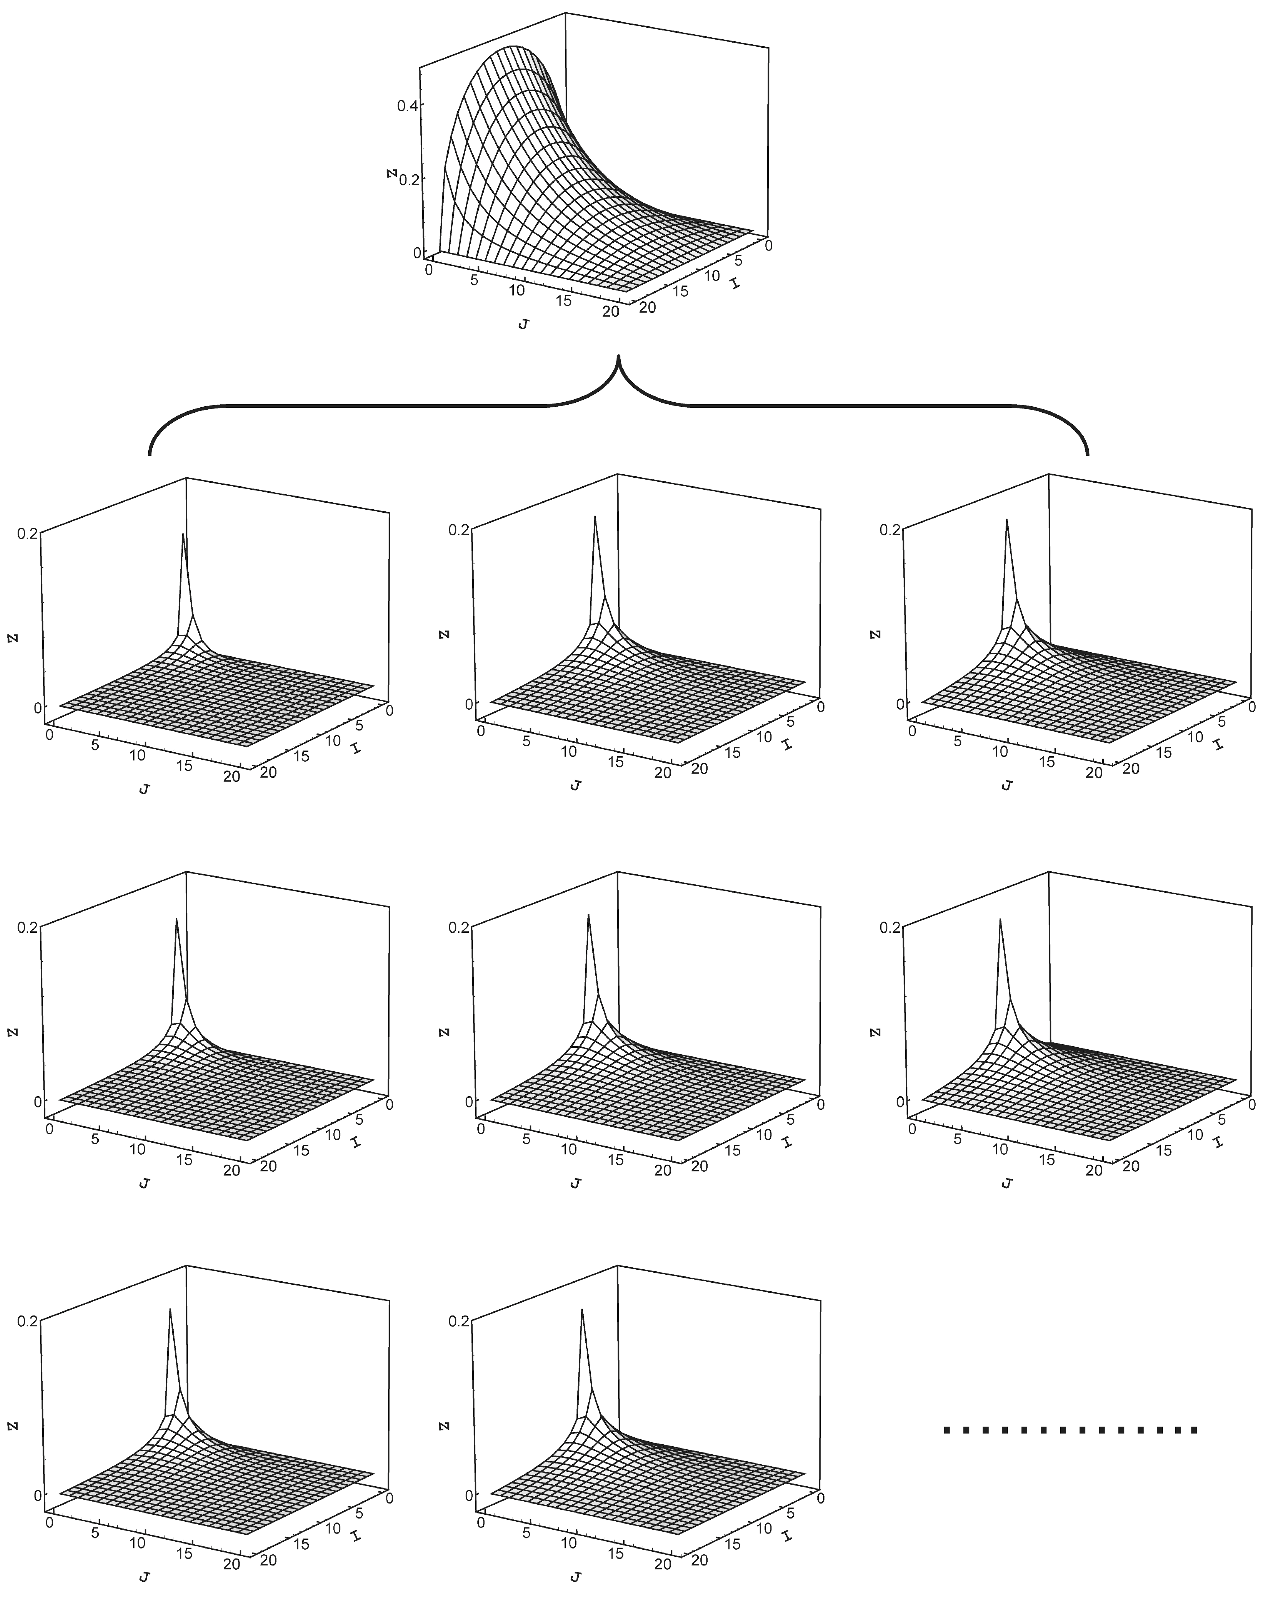
\includegraphics[width=6in]{../figures/SES/example_Laplace+Robin+Dirichlet.pdf}%pdf
\caption{Laplace equation with Robin and Dirichlet boundary conditions}
\label{fig:example-Laplace-Robin-Dirichlet}
\end{figure}

The Robin Boundary condition is the linear combination of the Neumann and Dirichlet boundary condition:
\be
\n^2 \Phi(r)= 0 \hst \te{in} \hst \Omega
\hst \te{and} \hst
a \ \f{\p\Phi(r)}{\p n}+ b \ \Phi(r) = R(r) \hs{0.2in} \te{on} \hs{0.2in} \p\Omega
\label{eqn:Laplace-Robin}
\ee
where $a$ and $b$ are some constants. Similar to the superposition method for Laplace equation with Dirichlet or Neumann boundary condition, the solution based on fundamental solutions $\Phi^o_i$ to $W$ sets of Robin boundaries can be written as:
\be
\Phi = \sum_{i=1}^W r_i \Phi^o_i
\ee
Consider a Laplace equation in a square domain with a Robin boundary on one side and Dirichlet boundary equals zero on the others:
\ben
\n^2 \Phi(x,y)=0, \hst 0< x, y <2;
\een
\be
\lt. -\f{\p \Phi}{\p x} \rt|_{(o,y)}+ \Phi(0,y) = 1,\hst \Phi(2,y)=\Phi(x,0)=\Phi(x,2)=0
\ee
Let $\Delta x=\Delta y=0.1$,the fundamental solution $\Phi^o_j$ is computed by setting the Robin boundary equals unity at $(x,y)=(0,j\Delta y)$ and equals zero otherwise:
\ben
\n^2 \Phi^o_j(x,y)=0, \hst 0< x, y <2 ; \hst \Phi(20,y)=\Phi(x,0)=\Phi(x,20)=0, \nonumber
\een
\be
\lt. \f{\p \Phi^o_j}{\p x} \rt|_{(0,y)}+ \Phi(0,y) = \lt\{
\baa{ccc}
0 \hst & if & y\neq j\Delta y \\
1 \hst & if & y = j\Delta y
\eaa
\rt.
\ee
The solution $\Phi$ can be constructed by superposing all the fundamental solutions as shown in Figure \ref{fig:example-Laplace-Robin-Dirichlet}.


\subsection{Poisson Equation with Dirichlet Boundary Condition}

\begin{figure}[htbp]
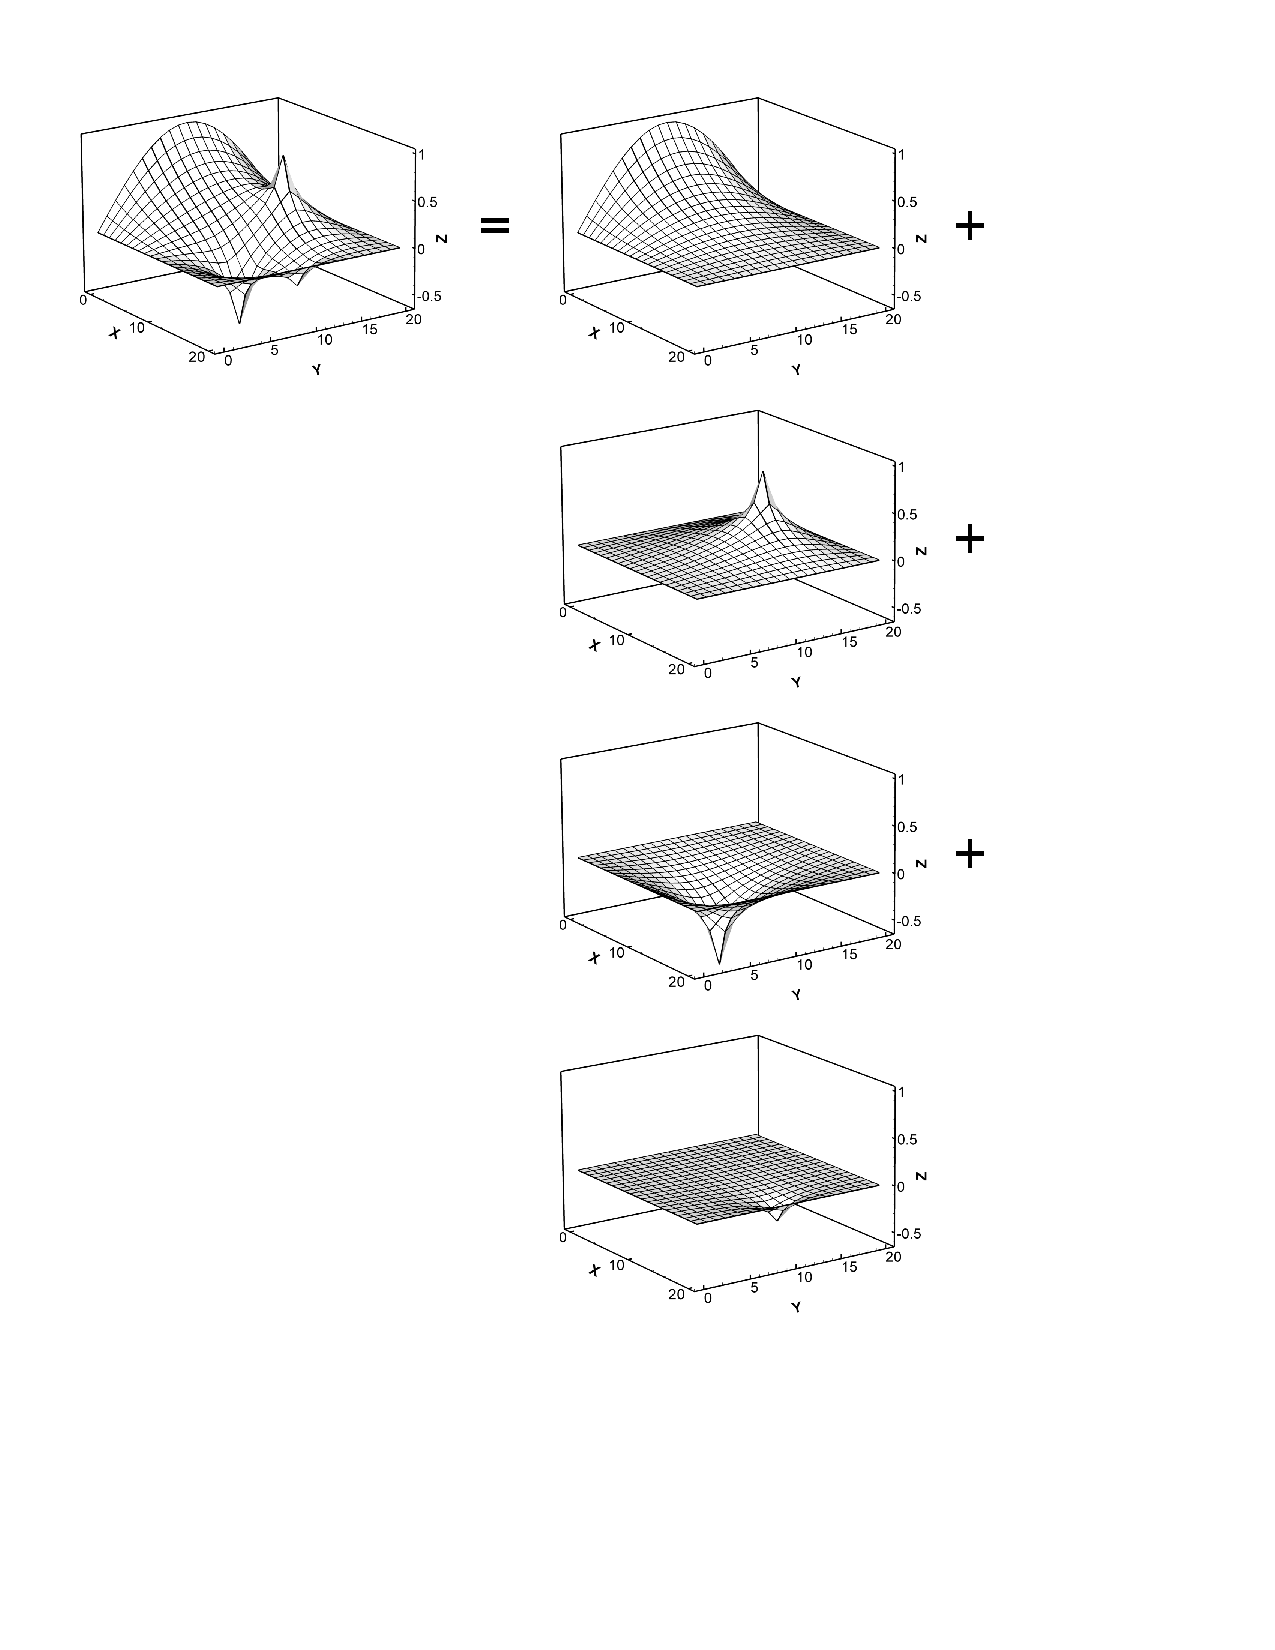
\includegraphics[width=6in]{../figures/SES/example_Laplace+Poisson.pdf}
\caption{Poisson equation with Dirichlet boundary condition}
\label{fig:example-Laplace-Poisson}
\end{figure}


Previous discussion of Laplace equation is limited by the zero source term, now we will drop the limitation and extend to the Poisson equation.
The Poisson equation with the Dirichlet boundary condition can be written as:
\ba
\n^2 \Phi(r)= S(r) \hst \te{in} \hst \Omega \hst \te{and} \hst
\Phi(r)= D(r) \hst \te{on} \hst \p \Omega
\label{eqn:Poisson-Dirichlet}
\ea

With the help of the superposition principle, the solution to the above equation can be decomposed into two parts: $\Phi_S$ and $\Phi_D$; where $\Phi_D$ is the solution to the Laplace equation with the specified Dirichlet boundary condition $D$, and $\Phi_S$ is the solution to the Poisson equation with the specified source term $S$ and the boundary value equals to zero:
\be
\Phi = \Phi_L + \Phi_P
\ee
\be
\n^2 \Phi_L(r)= 0 \hst \te{in} \hst \Omega
\hsand
\Phi_L(r)= D(r) \hs{0.2in} \te{on} \hs{0.2in} \p\Omega
\ee
\be
\n^2 \Phi_P(r)= S(r) \hst \te{in} \hst \Omega
\hsand
\Phi_P(r)= 0 \hs{0.2in} \te{on} \hs{0.2in} \p\Omega
\ee
The Laplace equation with the Dirichlet boundary condition is already discussed. Here we will focus on constructing the solution $\Phi_P$.

The system of equations resulted from the finite difference method for $\Phi_P$ can be written as:
\be
\left[
\baa{cccc}
a_{11} & a_{12} & \ldots & a_{1N} \\
a_{21} & a_{22} & \ldots & a_{2N} \\
\vdots & \vdots & \ddots & \vdots \\
a_{N1} & a_{N2} & \ldots & a_{NN}
\eaa
\right]\left[
\baa{c}
\phi_{P1} \\ \phi_{P2} \\ \vdots \\
\phi_{PN}
\eaa
\right]=
\left[
\baa{c}
s_{1} \\ s_{2} \\ \vdots \\
s_{N}
\eaa
\right]
\ee
or
\be
A \Phi_P = S
\ee
We can choose $N$ sets of the fundamental source terms that are zero everywhere except at the $i-th$ point the source equals unity:
\be
S^o_i=( s^o_{i1}, \ s^o_{i2}, \ \cdots, \ s^o_{iN}  )^T \hst
s^o_{ij} = \left\{
\baa{ccc}
0 \hst & if & j\neq i \\
1 \hst & if & j= i
\eaa
\right.
\ee
The corresponding numerical fundamental solutions are computed to satisfy the Poisson equation with the above source terms:
\be
\Phi^o_{Pi} = (\phi^o_{Pi1}, \ \phi^o_{Pi2}, \ \cdots, \ \phi^o_{PiN})^T \\
\ee
\be
\n^2 (\phi^o_{Pi1}, \ \phi^o_{Pi2}, \ \cdots, \ \phi^o_{PiN})^T = ( s^o_{i1}, \ s^o_{i2}, \ \cdots, \ s^o_{iN}  )^T
\ee
The solution $\Phi_P$ can be constructed as:
\be
\left[
\baa{c}
\phi_{P1} \\ \phi_{P2} \\ \vdots \\
\phi_{PN}
\eaa
\right]=\sum_{i=1}^N
S_{i}
\left[
\baa{c}
\phi^o_{Pi1} \\ \phi^o_{Pi2} \\ \vdots \\
\phi^o_{PiN}
\eaa
\right]
\ee
Combined with the solution $\Phi_L$, the solution $\Phi$ is:
\be
\Phi = \sum_{i=1}^N s_i \Phi^o_{Pi} + \sum_{i=1}^W d_i \Phi^o_{Li}
\ee

\subsection{Poisson Equation with Neumann Boundary Condition}

\begin{figure}[htbp]
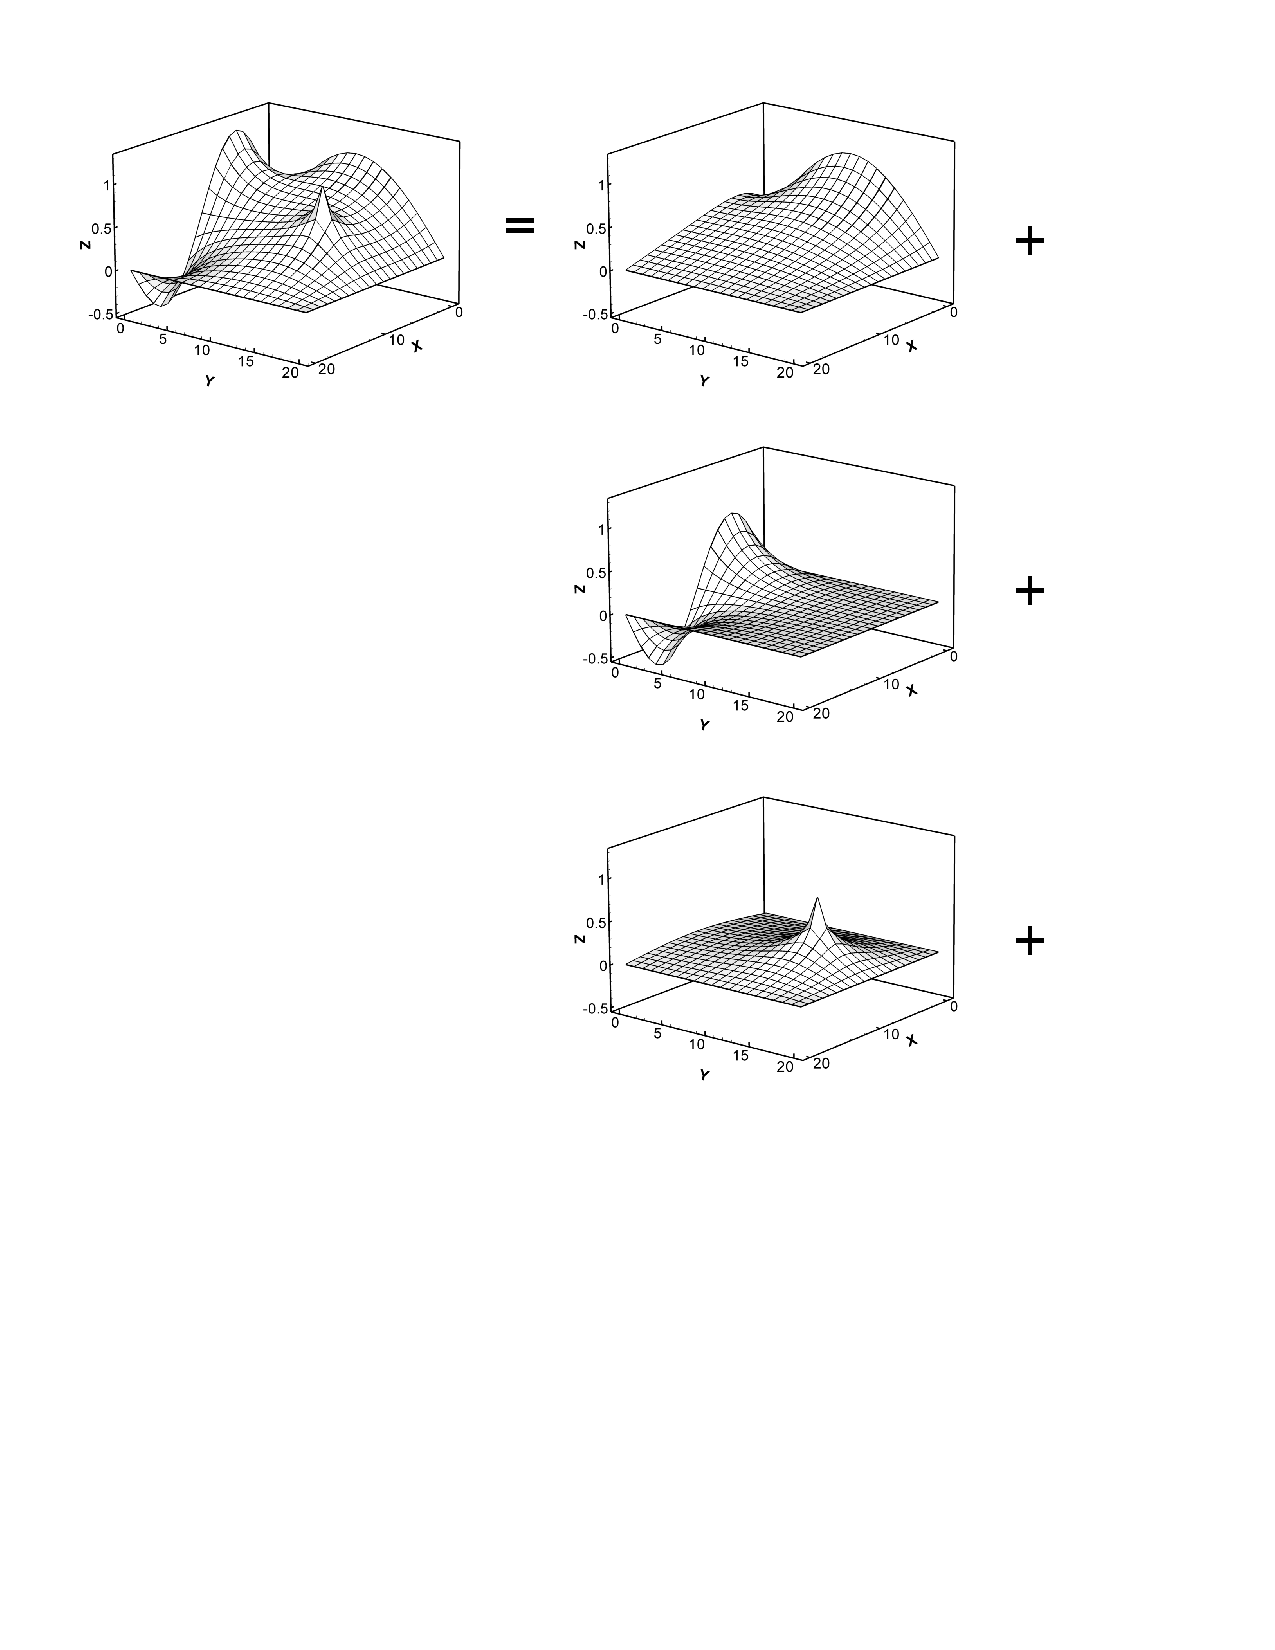
\includegraphics[width=6in]{../figures/SES/example_Laplace+Poisson+Neumann.pdf}
\caption{Poisson equation with Neumann and Dirichlet boundary conditions}
\label{fig:example-Laplace-Poisson-Neumann}
\end{figure}


The Poisson equation with the Neumann boundary condition can be written as:
\ba
\n^2 \Phi(r)= S(r) \hst \te{in} \hst \Omega \hsand
\f{\p\Phi(r)}{\p n}= Q(r) \hst \te{on} \hst \p \Omega
\ea
Similar to the last section, the Poisson equation with the Neumann boundary condition can be decomposed into $\Phi_Q$, the solution to the Laplace equation with the specified Neumann boundary condition $Q$; and $\Phi_P$, the solution to the Poisson equation with the specified source $S$ and the derivative on the boundary equals to zero:
\be
\Phi=\Phi_Q + \Phi_P
\ee
\be
\n^2 \Phi_Q(r)= 0 \hst \te{in} \hst \Omega
\hsand
\f{\p\Phi_Q(r)}{\p n}= Q(r) \hson \p\Omega
\ee
\be
\n^2 \Phi_P(r)= S(r) \hsin \Omega
\hsand
\Phi_P(r)= 0 \hson \p\Omega
\ee
The solution for $\Phi_Q$ is shown before, here we will find the superposed solution for $\Phi_P$. The discretized system of equations for $\Phi_P$ can be written as:
\be
A_P \ \Phi_P = S
\ee
The fundamental source terms are chosen as:
\be
S^o_i=( s^o_{i1}, \ s^o_{i2}, \ \cdots, \ s^o_{iN}  )^T \hst
s^o_{ij} = \left\{
\baa{ccc}
0 \hst & if & j\neq i \\
1 \hst & if & j= i
\eaa
\right.
\ee
The corresponding fundamental solutions are:
\be
\Phi^o_{Pi} = (\phi^o_{Pi1}, \ \phi^o_{Pi2}, \ \cdots, \ \phi^o_{PiN})^T \\
\ee
\be
A_P  \ \Phi^o_{Pi} =S^o_i
\ee
Therefore the general solution $\Phi_P$ can be constructed from those fundamental solutions as:
\be
\Phi_P = \sum_{i=1}^N s_i \ \Phi^o_{Pi}
\ee
Combined with the solution $\Phi_Q$, the solution $\Phi$ is:
\be
\Phi = \sum_{i=1}^N s_i \ \Phi^o_{Pi} + \sum_{i=1}^W q_i \ \Phi^o_{Qi}
\ee
A Poisson equation in a square domain with a point source, sinusoidal Neumann boundary, and sinusoidal Dirichlet boundary can be written as:
\ben
\n^2 \Phi(x,y)=S(x,y), \hst 0< x, y <20;
\een
\be
\Phi(0,y)= sin(2 \pi \f{y}{20}),\hst \lt.\f{\p\Phi}{\p y} \rt|_{(x,0)}=sin(2 \pi \f{y}{40}), \hst \Phi(20,y)=\Phi(x,20)=0;
\ee
\ben
S(x,y)= \left\{
\baa{cl}
1 \hst & if \hst (x,y) =(10,14) \\
0 \hst & otherwise
\eaa
\rt.
\een
The solution to the above equation can be decomposed into three parts: $\Phi_P$, the solution to the Poisson equation with Dirichlet and Neumann boundary equals zero; $\Phi_L$, the solution to the Laplace equation with Dirichlet boundary equals the specified value and Neumann boundary equals zero; and $\Phi_Q$, the solution to the Laplace equation with Neumann boundary equals the specified value and Dirichlet boundary equals zero:
\ben
\n^2 \Phi_P(x,y)=S(x,y), \hst 0< x, y <20;
\een
\be
\Phi_P(0,y)= 0, \hst \lt. \f{\p \Phi_P}{\p x} \rt|_{(x,0)}=0, \hst \Phi_P(20,y)=\Phi_P(x,20)=0
\ee
\ben
\n^2 \Phi_Q(x,y)=0, \hst 0< x, y <20;
\een
\be
\Phi_Q(0,y)= 0,\hst \lt.\f{\p\Phi}{\p y} \rt|_{(x,0)}=sin(2 \pi \f{y}{40}), \hst \Phi_P(20,y)=\Phi_P(x,20)=0
\ee
\ben
\n^2 \Phi_L(x,y)=0, \hst 0< x, y <20;
\een
\be
\Phi_L(0,y)= sin(2 \pi \f{y}{20}),\hst \lt.\f{\p\Phi_L}{\p y} \rt|_{(x,0)}=0, \hst \Phi_L(20,y)=\Phi_L(x,20)=0
\ee
The solution $\Phi$ can be constructed by superposing the solutions $\Phi_P$, $\Phi_Q$, and $\Phi_L$ as shown in Figure \ref{fig:example-Laplace-Poisson-Neumann}.


\section{Conclusion}
For $N$-points discretization of the domain $\Omega$ , there are $N$ elemental functions $\Phi^o_i$ and one base function $B$ need to be solved.
If a solver with $O(N)$ complexity is used, it will take $O(N^2)$ operations to build the elemental functions. It takes another $N$ multiplications and $N$ additions to construct the solution at one single point from the elemental functions. Therefore it takes $2N \times N$ operations to construct the solution for the whole domain. If the solutions to the Poisson equation with different source terms are required on the same grid for $T$ times, the average operation counts for constructing the solution at one single point is $O({N^2}/{T}) + 2N$, while the solution for the whole domain takes $O({N^2}/{T}) + 2N^2$ operations.
Compared with the well-known Multigrid method that requires only $O(N)$ operations, the superposition method has no advantage except for large $T$ and few point solutions. When $O(T/N)>>1$, the complexity of the superposition method for $k$ point solution becomes $O(kN)$. % when $T$ approaches infinity, the complexity will be asymptotic to $2kN$
\be
\mathop {\lim }\limits_{T \to \infty} O({N^2}/{T}) + 2kN = 2kN
\ee
If those $k$ points solutions are further approximated locally from source terms at $m$ points instead of the whole domain $N$ points, then the complexity will be reduced to $2km$.

The storage for the $N$ elemental functions is $O(N^2)$, which is pretty large compared with the Multigrid solver that need only $O(N)$ storage. However, the required storage for $k$ points solutions approximated from $m$ points source terms reduced to $O(km)$ because the number of elemental functions needed is $m$ and these $m$ function values are only needed at those $k$ points.


%Even though the problem of interest may be bounded or semi-bounded and boundary conditions of the governing equation may be specified, the Green's function is usually solved without boundary condition. In other words, the boundary of Green's function is located at infinity.

\normalsize
\chapter{Constrained Interpolation Profile Method}
\label{appendix:CIP}

The constrained interpolation profile method is proposed by Yabe et. al.
\cite{Yabe1991A, Yabe1991B, Yabe01, Xiao1999}. The scalar transport equations used in the unsteady non-hydrostatic flow model of Chapter \ref{chapter:FlowModel} are published by Xiao et. al. \cite{Xiao1999}. The two and three-dimensional cases in the paper \cite{Xiao1999} are listed here for completeness.


\section{ Two-Dimensional Case }
\be
f_i^{n+1}=F(x_i-u\Delta t, y_j-v\Delta t)
\ee
\be
\p_x f_i^{n+1}=\p_x F(x_i-u\Delta t, y_j-v\Delta t)-\p_x u \cdot \p_x f - \p_x v \cdot \p_y f
\ee
\be
\p_y f_i^{n+1}=\p_y F(x_i-u\Delta t, y_j-v\Delta t)-\p_y u \cdot \p_x f - \p_y v \cdot \p_y f
\ee
where
\be
F_{i,j}(x,y)=
\left[{\sum_{\scriptstyle 0\le {l_x}+{l_y}\le 3}}C_{{l_x},{l_y}}(x-x_i)^{l_x}(y-y_j)^{l_y}\right]
\left[\sum_{\scriptstyle 0\le p+q\le 1} \alpha_{p,q}\beta_{p,q}(x-x_i)^p(y-y_j)^q \right]^{-1}
\ee

\begin{eqnarray}
C_{2,1}&=&[\alpha_{0,1}\beta_{0,1}f_{i-isign,j}+(1+\alpha_{1,0}\beta_{1,0}\Delta_x)d_{yi-isign,j}-C_{0,1}]/\Delta_x^2 -C_{1,1}/\Delta_x \\
           C_{1,2}&=&[\alpha_{1,0}\beta_{1,0}f_{i,j-jsign}+(1+\alpha_{0,1}\beta_{0,1}\Delta_y)d_{xi,j-jsign}-C_{1,0}]/\Delta_y^2  -C_{1,1}/\Delta_y \\
           C_{1,1}&=&[\alpha_{0,1}\beta_{0,1}f_{i-isign,j}+(1+\alpha_{1,0}\beta_{1,0}\Delta_x)d_{yi-isign,j}]/\Delta_x  \nonumber \\
                  & &+[\alpha_{1,0}\beta_{1,0}f_{i,j-jsign}+(1+\alpha_{0,1}\beta_{0,1}\Delta_y)d_{xi,j-jsign}]/\Delta_y  \nonumber \\
                  & &+[C_{0,0}-({\sum_{\scriptstyle 0\le p+q\le 1}} \alpha_{p,q}\beta_{p,q}{\Delta_x}^p{\Delta_y}^q)f_{i-isign,j-jsign}]/\Delta_x/\Delta_y  \nonumber \\
                  & &+C_{3,0}\Delta_x^2/\Delta_y+C_{0,3}\Delta_y^2/\Delta_x+C_{2,0}\Delta_x/\Delta_y+C_{0,2}\Delta_y/\Delta_x \\
           C_{3,0}&=&[(1+\alpha_{1,0}\beta_{1,0}\Delta_x)(d_{xi-isign,j}-S_x)+d_{xi,j}-S_x ]/\Delta_x^2\\
           C_{0,3}&=&[(1+\alpha_{0,1}\beta_{0,1}\Delta_y)(d_{yi,j-jsign}-S_y)+d_{yi,j}-S_y ]/\Delta_y^2\\
           C_{2,0}&=&[(1+\alpha_{1,0}\beta_{1,0}\Delta_x)f_{i-isign,j}-C_{0,0}-C_{1,0}\Delta_x]/\Delta_x^2-C_{3,0}\Delta_x,\\
           C_{0,2}&=&[(1+\alpha_{0,1}\beta_{0,1}\Delta_y)f_{i,j-jsign}-C_{0,0}-C_{0,1}\Delta_y]/\Delta_y^2-C_{0,3}\Delta_y\\
           C_{1,0}&=&d_{xi,j} +\alpha_{1,0}\beta_{1,0}C_{0,0} \\
           C_{0,1}&=&d_{yi,j} +\alpha_{0,1}\beta_{0,1}C_{0,0} \\
           C_{0,0}&=&f_{i,j}\\
\beta _{0,0}&=&1.0\\
\beta _{1,0}&=&[|(S_x-d_{xi,j})/(d_{xi-isign,j}-S_x)|-1]/\Delta_x\\
\beta _{0,1}&=&[|(S_y-d_{yi,j})/(d_{yi,j-jsign}-S_y)|-1]/\Delta_y\\
           S_x &=& (f_{i-isign,j}-f_{i,j})/\Delta_x\\
           S_y &=& (f_{i,j-jsign}-f_{i,j})/\Delta_y\\
       d_{xi,j} &=& \partial_x f_{i,j}\\
       d_{yi,j} &=& \partial_y f_{i,j}\\
\Delta _x &=& x_{i-isign}-x_{i}\\
\Delta _y &=& y_{j-jsign}-y_{j}
\end{eqnarray}
\begin{eqnarray}
isign &=& \left\{ \begin{array}{ll}
                  -1 \ \ if \ \ u_{i,j} \leq 0 \\
                   1 \ \ if \ \ u_{i,j} > 0
                   \end{array} \right. \\
jsign &=& \left\{ \begin{array}{ll}
                  -1 \ \ if \ \ v_{i,j} \leq 0  \\
                   1 \ \ if \ \ v_{i,j} > 0
                   \end{array} \right.\\
\alpha_{1,0} &=& \left\{ \begin{array}{ll}
                   1 \ \ if \ \ d_{xi,j}\cdot d_{xi-isign,j} < 0 \\
                   0 \ \ if \ \ d_{xi,j}\cdot d_{xi-isign,j} \geq 0
                   \end{array} \right.\\
\alpha_{0,1} &=& \left\{ \begin{array}{ll}
                   1 \ \ if \ \ d_{yi,j}\cdot d_{yi,j-jsign} < 0 \\
                   0 \ \ if \ \ d_{yi,j}\cdot d_{yi,j-jsign} \geq 0
                   \end{array} \right.
\end{eqnarray}


\section {Three-Dimensional Case }
\be
f_i^{n+1}=F(x_i-u\Delta t, y_j-v\Delta t, y_k-w\Delta t)
\ee
\be
\p_x f_i^{n+1}=\p_x F(x_i-u\Delta t, y_j-v\Delta t, y_k-w\Delta t)-\p_x u \cdot \p_x f - \p_x v \cdot \p_y f - \p_x w \cdot \p_z f
\ee
\be
\p_y f_i^{n+1}=\p_y F(x_i-u\Delta t, y_j-v\Delta t, y_k-w\Delta t)-\p_y u \cdot \p_x f - \p_y v \cdot \p_y f - \p_y w \cdot \p_z f
\ee
\be
\p_z f_i^{n+1}=\p_z F(x_i-u\Delta t, y_j-v\Delta t, y_k-w\Delta t)-\p_z u \cdot \p_x f - \p_z v \cdot \p_y f - \p_z w \cdot \p_z f
\ee
where
\ba
F_{i,j,k}(x,y,z)= \left[{\sum_{\scriptstyle 0\le p+q+r\le 1} \alpha_{p,q,r}\beta_{p,q,r}(x-x_i)^p(y-y_j)^q(z-z_k)^r} \right]^{-1} \times \nonumber \\
\left[{\sum_{\scriptstyle 0\le {l_x}+{l_y}+{l_z}\le 3}}C_{{l_x},{l_y},{l_z}}(x-x_i)^{l_x}(y-y_j)^{l_y}(z-z_k)^{l_z}\right]
\ea
\begin{eqnarray}
           C_{1,1,1}&=&{\bigg[}{\bigg(}{\sum_{\scriptstyle 0\le p+q+r\le 1}} \alpha_{p,q,r}\beta_{p,q,r}\Delta_x^p\Delta_y^q\Delta_z^r{\bigg)}f_{i-isign,j-jsign,k-ksign} \nonumber \\
                  & &-C_{0,0,0}-C_{1,0,0}\Delta_x-C_{0,1,0}\Delta_y-C_{0,0,1}\Delta_z \nonumber \\
                  & &-C_{1,1,0}\Delta_x\Delta_y-C_{1,0,1}\Delta_x\Delta_z-C_{0,1,1}\Delta_y\Delta_z-C_{2,1,0}\Delta_x^2\Delta_y \nonumber \\
                  & &-C_{1,2,0}\Delta_x\Delta_y^2-C_{2,0,1}\Delta_x^2\Delta_z-C_{1,0,2}\Delta_x\Delta_z^2-C_{0,2,1}\Delta_y^2\Delta_z \nonumber \\
                  & &-C_{0,1,2}\Delta_y\Delta_z^2-C_{2,0,0}\Delta_x^2-C_{0,2,0}\Delta_y^2-C_{0,0,2}\Delta_z^2 \nonumber \\
                  & &-C_{3,0,0}\Delta_x^3-C_{0,3,0}\Delta_y^3-C_{0,0,3}\Delta_z^3{\bigg]}{\big /}(\Delta_x\Delta_y\Delta_z)
\end{eqnarray}
\begin{eqnarray}
           C_{2,1,0}&=&{\bigg[}{\bigg(}{\sum_{\scriptstyle 0\le p+q\le 1}} \alpha_{p,q,0}\beta_{p,q,0}\Delta_x^p\Delta_y^q{\bigg)}f_{i-isign,j-jsign,k} \nonumber \\
                  & &-(1+\alpha_{0,1,0}\beta_{0,1,0}\Delta_y)\Delta_xd_{xi,j-jsign,k}-\alpha_{1,0,0}\beta_{1,0,0}\Delta_xf_{i,j-jsign,k} \nonumber \\
                  & &+C_{1,0,0}\Delta_x-\zeta_{xy}{\bigg]}{\big /}(\Delta_x^2\Delta_y)
\end{eqnarray}
\begin{eqnarray}
           C_{1,2,0}&=&{\bigg[}{\bigg(}{\sum_{\scriptstyle 0\le p+q\le 1}} \alpha_{p,q,0}\beta_{p,q,0}\Delta_x^p\Delta_y^q{\bigg)}f_{i-isign,j-jsign,k} \nonumber \\
                  & &-(1+\alpha_{1,0,0}\beta_{1,0,0}\Delta_x)\Delta_yd_{yi-isign,j,k}-\alpha_{0,1,0}\beta_{0,1,0}\Delta_yf_{i-isign,j,k} \nonumber \\
                  & &+C_{0,1,0}\Delta_y-\zeta_{xy}{\bigg]}{\big /}(\Delta_x\Delta_y^2),
\end{eqnarray}
\begin{eqnarray}
           C_{1,1,0}&=&{\bigg[}{\bigg(}{\sum_{\scriptstyle 0\le p+q\le 1}} \alpha_{p,q,0}\beta_{p,q,0}\Delta_x^p\Delta_y^q{\bigg)}f_{i-isign,j-jsign,k} \nonumber \\
                  & &-C_{2,1,0}\Delta_x^2\Delta_y-C_{1,2,0}\Delta_x\Delta_y^2-\zeta_{xy}{\bigg]}{\big /}(\Delta_x\Delta_y)
\end{eqnarray}
\begin{eqnarray}
           C_{2,0,1}&=&{\bigg[}{\bigg(}{\sum_{\scriptstyle 0\le p+r\le 1}} \alpha_{p,0,r}\beta_{p,0,r}\Delta_x^p\Delta_z^r{\bigg)}f_{i-isign,j,k-ksign} \nonumber \\
                  & &-(1+\alpha_{0,0,1}\beta_{0,0,1}\Delta_z)\Delta_xd_{xi,j,k-ksign}-\alpha_{1,0,0}\beta_{1,0,0}\Delta_xf_{i,j,k-ksign} \nonumber \\
                  & &+C_{1,0,0}\Delta_x-\zeta_{xz}{\bigg]}{\big /}(\Delta_x^2\Delta_z)
\end{eqnarray}
\begin{eqnarray}
           C_{1,0,2}&=&{\bigg[}{\bigg(}{\sum_{\scriptstyle 0\le p+r\le 1}} \alpha_{p,0,r}\beta_{p,0,r}\Delta_x^p\Delta_z^r{\bigg)}f_{i-isign,j,k-ksign} \nonumber \\
                  & &-(1+\alpha_{1,0,0}\beta_{1,0,0}\Delta_x)\Delta_zd_{zi-isign,j,k}-\alpha_{0,0,1}\beta_{0,0,1}\Delta_zf_{i-isign,j,k} \nonumber \\
                  & &+C_{0,0,1}\Delta_z-\zeta_{xz}{\bigg]}{\big /}(\Delta_x\Delta_z^2)
\end{eqnarray}
\begin{eqnarray}
           C_{1,0,1}&=&{\bigg[}{\bigg(}{\sum_{\scriptstyle 0\le p+r\le 1}} \alpha_{p,0,r}\beta_{p,0,r}\Delta_x^p\Delta_z^r{\bigg)}f_{i-isign,j,k-ksign} \nonumber \\
                  & &-C_{2,0,1}\Delta_x^2\Delta_z-C_{1,0,2}\Delta_x\Delta_z^2-\zeta_{xz}{\bigg]}{\big /}(\Delta_x\Delta_z)
\end{eqnarray}
\begin{eqnarray}
           C_{0,2,1}&=&{\bigg[}{\bigg(}{\sum_{\scriptstyle 0\le q+r\le 1}} \alpha_{0,q,r}\beta_{0,q,r}\Delta_y^q\Delta_z^r{\bigg)}f_{i,j-jsign,k-ksign} \nonumber \\
                  & &-(1+\alpha_{0,0,1}\beta_{0,0,1}\Delta_z)\Delta_yd_{yi,j,k-ksign}-\alpha_{0,1,0}\beta_{0,1,0}\Delta_yf_{i,j,k-ksign} \nonumber \\
                  & &+C_{0,1,0}\Delta_y-\zeta_{yz}{\bigg]}{\big /}(\Delta_y^2\Delta_z)
\end{eqnarray}
\begin{eqnarray}
           C_{0,1,2}&=&{\bigg[}{\bigg(}{\sum_{\scriptstyle 0\le q+r\le 1}} \alpha_{0,q,r}\beta_{0,q,r}\Delta_y^q\Delta_z^r{\bigg)}f_{i,j-jsign,k-ksign} \nonumber \\
                  & &-(1+\alpha_{0,1,0}\beta_{0,1,0}\Delta_y)\Delta_zd_{zi,j-jsign,k}-\alpha_{0,0,1}\beta_{0,0,1}\Delta_zf_{i,j-jsign,k} \nonumber \\
                  & &+C_{0,0,1}\Delta_z-\zeta_{yz}{\bigg]}{\big /}(\Delta_y\Delta_z^2)
\end{eqnarray}
\begin{eqnarray}
           C_{0,1,1}&=&{\bigg[}{\bigg(}{\sum_{\scriptstyle 0\le q+r\le 1}} \alpha_{0,q,r}\beta_{0,q,r}\Delta_y^q\Delta_z^r{\bigg)}f_{i,j-jsign,k-ksign} \nonumber \\
                  & &-C_{0,2,1}\Delta_y^2\Delta_z-C_{0,1,2}\Delta_y\Delta_z^2-\zeta_{yz}{\bigg]}{\big /}(\Delta_y\Delta_z)
\end{eqnarray}
\begin{eqnarray}
           C_{2,0,0}&=&[(1+\alpha_{1,0,0}\beta_{1,0,0}\Delta_x)f_{i-isign,j,k}-C_{0,0,0}-C_{1,0,0}\Delta_x]/(\Delta_x^2) \nonumber \\
           & &-C_{3,0,0}\Delta_x
\end{eqnarray}
\begin{eqnarray}
           C_{0,2,0}&=&[(1+\alpha_{0,1,0}\beta_{0,1,0}\Delta_y)f_{i,j-jsign,k}-C_{0,0,0}-C_{0,1,0}\Delta_y]/(\Delta_y^2) \nonumber \\
           & &-C_{0,3,0}\Delta_y
\end{eqnarray}
\begin{eqnarray}
           C_{0,0,2}&=&[(1+\alpha_{0,0,1}\beta_{0,0,1}\Delta_z)f_{i,j,k-ksign}-C_{0,0,0}-C_{0,0,1}\Delta_z]/(\Delta_z^2) \nonumber \\
           & &-C_{0,0,3}\Delta_z
\end{eqnarray}
\begin{equation}
           C_{3,0,0}=[(1+\alpha_{1,0,0}\beta_{1,0,0}\Delta_x)(d_{xi-isign,j,k}-S_x)+d_{xi,j,k}-S_x]/(\Delta_x^2)
\end{equation}
\begin{equation}
           C_{0,3,0}=[(1+\alpha_{0,1,0}\beta_{0,1,0}\Delta_y)(d_{yi,j-jsign,k}-S_y)+d_{yi,j,k}-S_y]/(\Delta_y^2)
\end{equation}
\begin{equation}
           C_{0,0,3}=[(1+\alpha_{0,0,1}\beta_{0,0,1}\Delta_z)(d_{zi,j,k-ksign}-S_z)+d_{zi,j,k}-S_z]/(\Delta_z^2)
\end{equation}
\begin{equation}
           C_{1,0,0}=d_{xi,j,k} +\alpha_{1,0,0}\beta_{1,0,0}C_{0,0,0}
\end{equation}
\begin{equation}
           C_{0,1,0}=d_{yi,j,k} +\alpha_{0,1,0}\beta_{0,1,0}C_{0,0,0}
\end{equation}
\begin{equation}
           C_{0,0,1}=d_{zi,j,k} +\alpha_{0,0,1}\beta_{0,0,1}C_{0,0,0}
\end{equation}
\begin{equation}
           C_{0,0,0}=f_{i,j,k}
\end{equation}
\begin{equation}
           \beta _{0,0,0}=1.0
\end{equation}
\begin{equation}
           \beta _{1,0,0}=[|(S_x-d_{xi,j,k})/(d_{xi-isign,j,k}-S_x)|-1]/\Delta_x
\end{equation}
\begin{equation}
           \beta _{0,1,0}=[|(S_y-d_{yi,j,k})/(d_{yi,j-jsign,k}-S_y)|-1]/\Delta_y
\end{equation}
\begin{equation}
           \beta _{0,0,1}=[|(S_z-d_{zi,j,k})/(d_{zi,j,k-ksign}-S_z)|-1]/\Delta_z
\end{equation}
\begin{eqnarray}           \zeta_{xy}=C_{0,0,0}+C_{1,0,0}\Delta_x+C_{0,1,0}\Delta_y+C_{2,0,0}\Delta_x^2+C_{0,2,0}\Delta_y^2 +C_{3,0,0}\Delta_x^3+C_{0,3,0}\Delta_y^3\\
           \zeta_{xz}=C_{0,0,0}+C_{1,0,0}\Delta_x+C_{0,0,1}\Delta_z+C_{2,0,0}\Delta_x^2+C_{0,0,2}\Delta_z^2  +C_{3,0,0}\Delta_x^3+C_{0,0,3}\Delta_z^3\\
           \zeta_{yz}=C_{0,0,0}+C_{0,1,0}\Delta_x+C_{0,0,1}\Delta_z+C_{0,2,0}\Delta_y^2+C_{0,0,2}\Delta_z^2  +C_{0,3,0}\Delta_y^3+C_{0,0,3}\Delta_z^3
\end{eqnarray}
\ba
          &S_x=(f_{i-isign,j,k}-f_{i,j,k})/\Delta_x\\
          &S_y=(f_{i,j-jsign,k}-f_{i,j,k})/\Delta_y\\
          &S_z=(f_{i,j,k-ksign}-f_{i,j,k})/\Delta_z\\
      &d_{xi,j,k}=\partial_x f_{i,j,k}\\
          &d_{yi,j,k}=\partial_y f_{i,j,k}\\
          &d_{zi,j,k}=\partial_z f_{i,j,k}\\
          &\Delta _x=x_{i-isign}-x_{i}\\
          &\Delta _y=y_{j-jsign}-y_{j}\\
          &\Delta _z=z_{k-ksign}-z_{k}
\ea
\ba
isign=\left\{ \begin{array}{ll}
                  -1 \ \ if \ \ u_{i,j,k} \leq 0\\
                   1 \ \ if \ \ u_{i,j,k} > 0
                   \end{array} \right. \ea
\ba
jsign=\left\{ \begin{array}{ll}
                  -1 \ \ if \ \ v_{i,j,k} \leq 0\\
                   1 \ \ if \ \ v_{i,j,k} > 0
                   \end{array} \right. \ea
\ba
ksign=\left\{ \begin{array}{ll}
                  -1 \ \ if \ \ w_{i,j,k} \leq 0\\
                   1 \ \ if \ \ w_{i,j,k} > 0
                   \end{array} \right.
\ea
\begin{equation}
\alpha_{1,0,0}
                   =\left\{ \begin{array}{ll}
                   1 \ \ if \ \ d_{xi,j,k}\cdot d_{xi-isign,j,k} < 0\\
                   0 \ \ if \ \ d_{xi,j,k}\cdot d_{xi-isign,j,k} \geq 0
                   \end{array} \right.
\end{equation}
\begin{equation}
\alpha_{0,1,0}
                   =\left\{ \begin{array}{ll}
                   1 \ \ if \ \ d_{yi,j,k}\cdot d_{yi,j-jsign,k} < 0\\
                   0 \ \ if \ \ d_{yi,j,k}\cdot d_{yi,j-jsign,k} \geq 0
                   \end{array} \right.
\end{equation}
\begin{equation}
\alpha_{0,0,1}
                   =\left\{ \begin{array}{ll}
                   1 \ \ if \ \ d_{zi,j,k}\cdot d_{zi,j,k-ksign} < 0 \\
                   0 \ \ if \ \ d_{zi,j,k}\cdot d_{zi,j,k-ksign} \geq 0
                   \end{array} \right.
\end{equation}























\begin{comment}
\addcontentsline{toc}{section}{\hspace{-0.3in}\protect\numberline{}A.1 CIP}


A weak conservation technique is proposed to partially offset the loss or gain of the scalar transported by the CIP method:
\be
f^{n+1} = f^{n} + r(f^{*}-f^{n})
\ee
\be
r =  1-sign(f^{*}-f^{n})\left[\left(\f{\sum_i f^{*}}{\sum_i f_o}\right)^c-1\right]
\ee
where $f^{n}$ is the scalar at the previous time step, $f^*$ is the intermediate result, $\sum_i f_o$ is the reference sum, and $c$ is a user specified parameter ( $c\geq 0$)

%   ff(i,m,j) = ff(i,m,j) + (ff(i,m,j)-ff_0(i,m,j))*(1.0d0-total/total_ref)

%\section*{Einstein summation convention}
\end{comment}
